\documentclass{beamer}
\usetheme{CambridgeUS}
\usecolortheme{dolphin}
\setbeamertemplate{page number in head/foot}{}
\usepackage[utf8]{inputenc}
\usepackage{dirtytalk,amssymb,tikz,mathtools,amsmath, empheq}
\usepackage{stackengine}
\usepackage{stmaryrd}
\usepackage{graphicx}
\usepackage[noend]{algpseudocode,algorithm}
\usepackage{resizegather}
\usetikzlibrary{automata, positioning}
\graphicspath{ {./images/} }
\tikzset{->, initial text=$$}
\DeclareMathAlphabet{\mathpzc}{OT1}{pzc}{m}{it}

\makeatletter
\algrenewcommand\ALG@beginalgorithmic{\footnotesize}
\makeatother

%Information to be included in the title page:
\title[Parameter Invariant Monitoring for STL]{Parameter Invariant Monitoring for Signal Temporal Logic}
\subtitle{Nima Roohi, Ramneet Kaur, James Weimer, Oleg Sokolsky, Insup Lee}
\author{Manasvi Saxena}

%\setbeameroption{hide notes} % Only slides
%\setbeameroption{show only notes} % Only notes
%\setbeameroption{show notes on second screen=right} % Both
%\setbeamertemplate{note page}{\pagecolor{yellow!5}\insertnote}\usepackage{palatino}
\setbeamerfont{caption}{size=\scriptsize}
\date{}

%\newcommand\restr[2]{{% we make the whole thing an ordinary symbol
%  \left.\kern-\nulldelimiterspace % automatically resize the bar with \right
%  #1 % the function
%  \vphantom{\big|} % pretend it's a little taller at normal size
%  \right|_{#2} % this is the delimiter
%  }}
\renewcommand{\restriction}{\mathord{\upharpoonright}}
\newcommand{\always}[1]{\square_{#1}}
\newcommand{\eventually}[1]{\lozenge_{#1}}

\newcommand{\typeTime}{\mathbb{R}_{\geq 0}}
\newcommand{\typeReal}{\mathbb{R}}
\newcommand{\typeNat}{\mathbb{N}}
\newcommand{\typeProb}{\mathbb{P}}

\newcommand{\dom}{\text{dom}}

\newcommand{\accept}{\text{accept}}
\newcommand{\reject}{\text{reject}}
\newcommand{\unknown}{\text{unknown}}

\newcommand{\until}{\mathcal{U}}
\newcommand{\release}{\mathcal{R}}
\newcommand{\interval}{\mathcal{I}}
\newcommand{\observe}{\mathcal{O}}
\newcommand{\K}{\mathcal{K}}
\newcommand{\M}{\mathcal{M}}
\newcommand{\kk}{\mathcal{k}}
\newcommand{\A}{\mathcal{A}}

% text versions
\newcommand{\Z}{\text{Z}}
\newcommand{\f}{\text{f}}
\newcommand{\varT}{\text{t}}

%satisfaction
\newcommand{\discrete}{\raisebox{-0.1ex}{\scalebox{0.25}{\textrm{DSC}}}}
\newcommand{\cont}{\raisebox{-0.1ex}{\scalebox{0.25}{\textrm{CNT}}}}
\newcommand{\discreteSatisfy}{\ \stackMath\stackunder[0pt]{\vDash}{\hspace*{0.3em}\discrete}\ }
\newcommand{\contSatisfy}{\ \stackMath\stackunder[0pt]{\vDash}{\hspace*{0.3em}\cont}\ }
\newcommand{\robustAssign}{\; := \;}
\begin{document}

\frame{\titlepage}

\section{Introduction}
\subsection{Motivation}

\begin{frame}
    \frametitle{Motivations}

    Challenges in monitoring Real Time Systems -
    \begin{itemize}
        \item \textit{Partially Observable} States.
        \item \textit{Partially Observable} Traces.
        \item \textit{High Computation} Cost.
    \end{itemize}

    \pause

    Extends Parameter Invariant (PAIN) tests to -
    \begin{itemize}
        \item STL to support continuous systems
        \item Efficiently monitor STL online.
    \end{itemize}

\end{frame}

\begin{frame}
    \frametitle{Example}
    \framesubtitle{Monitoring a Diabetic Patient}

    STL formula, \say{If patient has a meal (M), then (s)he
    either recieved bolus $t_1$ units ago, or will recieve one in $t_2$ units}
        $$ \always{ [ t_1, \infty )}
    \left( \left (M > c_1 \right ) \to \eventually{\left(-t_1, t_2 \right)}
    \left( B > c_2 \right ) \right)$$.
    \pause
    \begin{itemize}
        \item \textit{State} variables not directly Observable.
        \item \textit{Output} variables affected by sensor and environment noise.
        \item Models are \textit{parametric}. Estimating (\textit{nuissance}) parameters is not
            feasible.
    \end{itemize}
\end{frame}
\begin{frame}
    \frametitle{Example}
    \framesubtitle{Monitoring a Diabetic Patient}

    STL formula, \say{If patient has a meal (M), then (s)he
    either recieved bolus $t_1$ units ago, or will recieve one in $t_2$ units}
    \begin{itemize}
        \item B (Bolus) is observable, but M (Meal) is not. Furthermore, B
            can be affected by noise.
        \pause
        \item Avoid relying on exact models of the system.
        \item Rely on \textit{probabilistic beliefs} about
            system state at a given point in time.
        \pause
        \item Furthermore, use \textit{maximally invariant} statistics
            to derive \textit{probabilistic beliefs}
    \end{itemize}
\end{frame}

\section{Preliminaries}
\subsection{Signal Temporal Logic (STL)}
\begin{frame}
    \frametitle{Signal Temporal Logic}
    \begin{block}{Signals}
        Given a finite set of variables $\Z$, signal
        $f : \typeTime \to \typeReal^{\Z}$ is a mapping
        from a point in \textit{time} to a \textit{valuation} of $\Z$.
    \end{block}
    \pause
    \begin{block}{Formulas over Signals}
        \begin{itemize}
            \item An formula $\theta : \typeReal^{\Z} \to \typeReal$
                  maps a \textit{valuation} to a real value.
            \item Function $\theta \circ f : \typeTime \to \typeReal$
                  maps points in time to values defined by $\theta$.
            \item At time $t \in \typeTime$, signal $f$ is \textit{true}
                w.r.t. $\theta$ whenever $\theta(f(t)) > 0 $.
                Conversely, $f$ is \textit{false} w.r.t $\theta$
                w.r.t. $\theta$ whenever $\theta(f(t)) < 0 $.
            \item Whenever, $\theta(f (t)) = 0$, value of $f$
                is \textit{unknown} on $\theta$ at time $t$.
            \item $\theta(f(t))$, is the \textit{robustness degree}.
                Larger \textit{robustness degree} values signify
                greater \textit{belief} about signal's adherence to $\theta$.
        \end{itemize}
    \end{block}
\end{frame}

\begin{frame}
    \frametitle{Signal Temporal Logic}
    \begin{block}{Syntax}
        \begin{itemize}
            \item $ \varphi ::= \top \;|\; \bot \;|\; \Theta \;|\; \neg \Theta
                \; | \; \varphi \wedge \varphi \;|\; \varphi\ \until_{\interval_{\geq 0}}\ \varphi
                \; | \; \varphi \release_{\interval_{\geq 0}} \varphi $
            \item $\eventually{\interval} \varphi \equiv \top\ \until_{\interval}\ \varphi$
            \item $\always{\interval} \varphi \equiv \bot \release_{\interval} \varphi$
            \item Law of Excluded Middle not assumed. Robustness 0 means
                signal neither satisfies nor not satisfies a formula.
                It is possible for $\varphi \vee \neg \varphi$ to not
                be true.
            \item Law of non contradiction still holds. It is not possible
                for both $\varphi$ and $\neg \varphi$ to be true.
        \end{itemize}
    \end{block}
\end{frame}

\begin{frame}
    \frametitle{Semantics}
    \begin{block}{Continuous Semantics}
        Given signal $f$ and a point in time $r : \typeTime$,
        Continuous time STL semantics are given inductively as -
        \begin{align*}
              f, r &\contSatisfy \top       \robustAssign \infty &
              f, r &\contSatisfy \bot       \robustAssign -\infty \\
              f, r &\contSatisfy \theta     \robustAssign \theta(f(r)) &
              f, r &\contSatisfy \neg\theta \robustAssign -\theta(f(r)) \\
        \end{align*}
        \vspace{-1.6cm}
        \begin{align*}
            f, r \contSatisfy \phi \vee \psi  \robustAssign  f, r \contSatisfy \phi \; \sqcup \; f,r \contSatisfy \psi \\
            f, r \contSatisfy \phi \wedge \psi  \robustAssign  f, r \contSatisfy \phi \; \sqcap \; f,r \contSatisfy \psi \\
        \end{align*}
    \end{block}
    where $\sqcup$ and $\sqcap$ represent $\text{sup}$, $\text{inf}$ respectively.
\end{frame}

\begin{frame}
    \frametitle{Semantics}
    \begin{block}{Continuous Semantics}
        Given signal $f$ and point in time $r : \typeTime$,
        Continuous time STL semantics are given inductively as -
        \begin{align*}
            f, r \contSatisfy \phi\ \until_{\interval}\ \psi
           \robustAssign \bigsqcup_{t: r+\interval}\left( f, t \contSatisfy \psi
           \sqcap \bigsqcap_{r \leq t' < t} \left( f, t' \contSatisfy \varphi
            \right ) \right) \\
            f, r \contSatisfy \phi\ \release_{\interval}\ \psi
           \robustAssign \bigsqcap_{t: r+\interval}\left( f, t \contSatisfy \psi
           \sqcup \bigsqcup_{r \leq t' < t} \left( f, t' \contSatisfy \varphi
            \right ) \right)
        \end{align*}
    \end{block}
    where $\sqcup$ and $\sqcap$ represent $\text{sup}$, $\text{inf}$ respectively.
\end{frame}

\begin{frame}
    \frametitle{Semantics}
    \begin{block}{Discrete Semantics}
        Given signal $f$ and sampling function $\tau : \typeNat
        \to \typeTime$, discrete time semantics for $g := f \circ \tau : \typeNat
        \to  \typeReal^{\Z}$ at step $n:\typeNat$ are given inductively as -
        \begin{align*}
              g, n &\discreteSatisfy \top       \robustAssign \infty &
              g, n &\discreteSatisfy \bot       \robustAssign -\infty \\
              g, n &\discreteSatisfy \theta     \robustAssign \theta(g(n)) &
              g, n &\discreteSatisfy \neg\theta \robustAssign -\theta(g(n)) \\
        \end{align*}
        \vspace{-1.6cm}
        \begin{align*}
            g, n \discreteSatisfy \phi \vee \psi  \robustAssign  g, n \discreteSatisfy \phi \; \sqcup \; g, n\discreteSatisfy \psi \\
            g, n \discreteSatisfy \phi \wedge \psi  \robustAssign  g, n \discreteSatisfy \phi \; \sqcap \; g, n \discreteSatisfy \psi \\
        \end{align*}
    \end{block}
    where $\sqcup$ and $\sqcap$ represent $\text{sup}$, $\text{inf}$ respectively.
\end{frame}

\begin{frame}
    \frametitle{Semantics}
    \begin{block}{Discrete Semantics}
        Given signal $f$ and sampling function $\tau : \typeNat
        \to \typeTime$, discrete time semantics for $g := f \circ \tau : \typeNat
        \to  \typeReal^{\Z}$ at step $n:\typeNat$ are given inductively as -
        \begin{align*}
            g, n \contSatisfy \phi\ \until_{\interval}\ \psi
            \robustAssign \bigsqcup_{i: \tau^{-1}(\tau((n) +\interval)}\left( g, i \contSatisfy \psi
           \sqcap \bigsqcap_{n \leq j < i} \left( g, j \contSatisfy \psi
            \right ) \right) \\
            g, n \contSatisfy \phi\ \release_{\interval}\ \psi
           \robustAssign \bigsqcap_{i: \tau^{-1}(\tau((n) +\interval)} \left( g, i \contSatisfy \psi
           \sqcup \bigsqcup_{n \leq j < i} \left( g, n' \contSatisfy \psi
            \right ) \right)
        \end{align*}
    \end{block}
    where $\sqcup$ and $\sqcap$ represent $\text{sup}$, $\text{inf}$ respectively.
\end{frame}

\begin{frame}
    \frametitle{Strengthening STL Formulas}
    For STL formula $\varphi$, and $\delta : \typeTime$,
    $\varphi^{\delta}$ (strengthening) is defined as -
    \begin{itemize}
        \item $\bot^{\delta} := \bot \;\;\;\; \top^{\delta} := \top   \;\;\;\; p^{\delta} := p
            \;\;\;\; (\neg p)^{\delta} := \neg p$
        \item $(\varphi \vee \psi)^{\delta} := \varphi^{\delta} \vee \psi^{\delta}
            \;\;\;\; (\varphi \wedge \psi)^{\delta} := \varphi^{\delta} \wedge \psi^{\delta}$
        \item $(\varphi\ \until_{\interval}\ \psi)^{\delta} := \varphi^{\delta} \
            \until_{\left (\underline{\interval} + \delta, \overline{\interval}
            - \delta \right)}\ \psi^{\delta}$
        \item $(\varphi\ \release_{\interval}\ \psi)^{\delta} := \varphi^{\delta} \
            \release_{\left ((\underline{\interval} - \delta)^{+}, \overline{\interval}
            + \delta \right)}\ \psi^{\delta}$
    \end{itemize}
    Intuitvely, strengthening slightly shortens (lengthens) intervals
    for $\until (\release) $. Along with conditions about the signal
    and sampling function, strengthening allows using discrete-time
    STL to reason about continuous-time STL.
\end{frame}

\begin{frame}
    \frametitle{Discrete to Continuous Time STL}
    Given signal $f$, formula $\varphi$, \textit{strictly increasing} sampling function
    $\tau$, where $\Delta \tau = \sqcup_{n : \typeNat}(\tau(n+1) - \tau(n))$,
    and $\delta : \typeTime$, where
    \begin{itemize}
        \item $\exists \lambda:\typeReal_{+}$ such
            that for $\theta : \Theta$, $\theta \circ f$ is
            $\lambda$-\textit{Lipschitz} continuous.
        \item $\delta$ is sufficiently large - $\lambda \Delta\tau < \delta$.
        \item Sampling is sufficient - $\Delta\tau < \frac{1}{3}
            \text{min}_{\interval:\interval_{\varphi}}(\overline{\interval} -
            \underline{\interval})$, where $\interval_{\varphi}$ are intervals
            in temporal operators of $\varphi$.
        \item Sampling started early - $\tau(0) < \Delta\tau$
    \end{itemize}
    guarantees the following hold -
    \begin{itemize}
        \item $f \circ \tau\ \discreteSatisfy\ \varphi^{\Delta\tau} \implies f
        \contSatisfy \varphi > 0 $.
        \item $f \circ \tau\ \discreteSatisfy\ \neg\varphi^{\Delta\tau} \implies f
        \contSatisfy \varphi < 0 $.
    \end{itemize}
    Instead of proving $f \contSatisfy \varphi > 0 $, prove
    $f, \tau \discreteSatisfy \varphi^{\Delta\tau} > \delta$.
\end{frame}

\subsection{Parameter Invariant Test Statisitc}

\begin{frame}
    \frametitle{Partially Observable States}
    Say we have test functions $\Theta$, signal $f$
    and sampling time $\tau$. For $\theta : \Theta$, $\theta \circ f$ cannot
    be directly observed.
    \begin{itemize}
        \item $\observe(\theta, f, t) = F\mu + \theta^+(f(t))G_0\rho_0
                + \theta^{-}(f(t))G_1\rho_1 + \sigma n$
        \item $Y$ is a set of \textit{observable} variables.
        \item $\mu : \dom(\mu) \to \typeReal, \rho_0 : \dom(\rho_i) \to
            \typeReal$ for $i \in \{0, 1\}$ are \textit{unknown nuissance} vectors.
        \item $F : \typeReal^{Y \times \dom(\mu)}$,
            $G_i : \typeReal^{Y \times \dom(\rho_i)}$ for $i \in \{0, 1\}$ are
            \textit{known signal matrices}.
        \item $\sigma$ is unkown noise multiplier, $n$ is random noise.
    \end{itemize}
\end{frame}

\subsection{Parameter Invariant Test Statisitc}

\begin{frame}
    \frametitle{Partially Observable States}
    \begin{itemize}
        \item It is assumed that for each \textit{test function}
            $\theta, \theta' \in \Theta$, $\theta \neq \theta' \implies
            Y_{\theta} \cup Y_{\theta'} = \emptyset$. In other words,
            different test functions use \textit{disjoint observable variables}.
        \item $\observe(f, t)$ - random variable corresponding to
            the observation of signal $f$ at time $t$ is \textit{uniquely determined}
            by $\observe(\theta, f, t)$ for each $\theta \in \Theta$.
    \end{itemize}
\end{frame}

\begin{frame}
    \frametitle{Invariance to Transformations}
    \begin{itemize}
        \item Given $\Omega$, the sampling space
            of a probabily-space and $\K \subseteq \Omega \to \Omega$
            a group of transformations.
        \item Let $\eta : \Omega \to \Omega'$ be a statistic.
        \item $\eta$ is said to be \textit{invariant} to
            group of transformations $\K$ iff
            $$ \forall \omega : \Omega, k : \K . \eta(\omega) = \eta(k(\omega))$$
        \item $\eta$ is said to be \textit{maximally invariant} to
            group of transformations $\K$ iff
            $$ \forall \omega, \omega' : \Omega . \eta(\omega) = \eta(\omega')
            \implies (\exists k : \K . \omega = k(\omega'))$$
    \end{itemize}
\end{frame}

\section{Parameter Invariance Monitoring For STL}
\subsection{Parameter Invariant Estimates}


\begin{frame}
\frametitle{Parameter Invariant Rosustness Estimation of Atomic Propositions}

    Suppose we have
    \begin{itemize}
        \item $\Omega_{f, \tau}: \typeNat \to \typeReal^{X}$, be the space
        of all observations at different sample time
        \item A sequence $x: \Omega_{f, \tau}$ test function $\theta \in \Theta$,
        error and indifference bounds $\alpha', \delta' :\typeReal^{+}$.
    \end{itemize}
    One can find a algorithm $\A(x, \tau, \theta, \alpha', \delta')$ such that -
    \begin{itemize}
        \item $\A$ is \textit{terminating} and returns value $r:\typeReal$.
        \item $\typeProb({\mid (\theta \circ f \circ \tau)(0) - r \mid > \delta'}) < \alpha'$
        \item The \textit{Probability} that $r$ (i.e. the \textit{robustness degree estimate}
            returned by $\A$) is more than $\delta'$ away from the real value of
            $f \circ \tau \discreteSatisfy \theta$ is less than $\alpha'$.
    \end{itemize}

\end{frame}

\begin{frame}

\frametitle{Parameter Invariant Robustness Estimation of Atomic Propositions}
    \begin{itemize}
        \item If \textit{statistic} used in $\A$ is \textit{Maximally
            Invariant}, then $r$, is invariant to nuissance parameters.
        \item A change in the \textit{noise} in sensor measurements
            will not affect $r$.
        \item Use $\A$ to obtain
             estimates that are \textit{(maximally) invariant}
             to nuissance parameters.
    \end{itemize}
\end{frame}

\begin{frame}

\frametitle{Parameter Invariant Estimation For Atomic Formulas}
    \begin{itemize}
        \item Using $\A$, we get \textit{robustness estimates}
            for atomic proposition $\theta \in \Theta$.
        \item Furthermore, if the estimate in $\A$ is derived
            using a \textit{maximally invariant} test statistic,
            the estimate is \textit{invariant} to \textit{nuissance}
            parameters (like noise).
        \item For example, robustness estimate will be invariant
            to sensor noise.
    \end{itemize}
\end{frame}

\begin{frame}
\frametitle{Parameter Invariant Estimation For Atomic Formulas}
    \begin{itemize}
        \item For given $\theta$, say $Y_{\theta}$ it the
            set of \textit{observable variables} of $\theta$.
        \item Let $\K_{\theta, f, \tau(n)} \subseteq \typeReal^{Y_{\theta}} \to \typeReal^{Y_{\theta}}$ be
            group of transformations affecting $\theta$.
        \item Let $\K_{f, \tau(n)} \subseteq \typeReal^{Y}\to \typeReal^{Y}$
           be group of transformations for $f$ at step $n$.
        \item For $v \in \typeReal^{Y}$, $\theta \in \Theta$, function
            $k \in  \K_{f, \tau(n)}$ maps $v \restriction^{Y_{\theta}}$ to some
            $k_{\theta}(v \restriction^{Y_{\theta}})$
           where $k_{\theta} \in \K_{\theta, f, \tau(n)}$.
       \item $\K_{f, \tau(n)}$ is \textit{completely determined}
           by $\K_{\theta, f, \tau(n)}$ since
            $\theta \neq \theta' \implies Y_{\theta}\cap Y_{\theta'}=\emptyset$

        %\item $\K_{f, \tau(n)} \subseteq \typeReal^{Y_{\theta}} \to
        %    \typeReal^{Y_{\theta}}$ is \textit{uniquely determined} by $\K_{\theta, f, \tau(n)}$
        %    since for $\theta_1, \theta_2 \in \Theta . Y_{\theta_1} \cap Y_{\theta_2} = \emptyset$.
        %\item Thus, if $\eta_{\theta, f, \tau(n)} : \typeReal^{Y} \to
        %    \Omega_{\theta, f, \tau(n)}$, such that $\eta_{\theta, f, \tau_n}$
        %    is invariant to $\K_{\theta, f, \tau_n}$

    \end{itemize}
\end{frame}

\begin{frame}
    \frametitle{Parameter Invariant Estimation For Atomic Formulas}
    \begin{itemize}
        \item Let $\eta_{\theta} : \typeReal^{Y_{\theta}} \to \typeReal$
            be statistics that produces \textit{estimates} for $\theta \in \Theta$.
        \item Define $\eta:\typeReal^{Y} \to \typeReal$ such
            that for $v \in \typeReal^{Y}$,
            $\eta(v) = \eta_{\theta}(v\restriction^{Y_{\theta}})$ for $\theta \in \Theta$.
        \item Suppose $\eta_{\theta}$ is invariant to $\K_{\theta, f, \tau(n)}$
            for each $\theta \in \Theta$.
        \item Formally, for $v : \typeReal^{Y}$ and
         $k_{\theta} \in \K_{\theta, f, \tau(n)}$,
            $\eta_{\theta}(v\restriction^{Y_{\theta}})
            = \eta_{\theta}(k_{\theta}(v\restriction^{Y_{\theta}}))$
        \item For $k \in \K_{f, \tau(n)}$, $k(v) =
            k_{\theta}(v\restriction^{Y_{\theta}})$.
        \item $\eta(k(v)) = \eta_{\theta}(k(v)) = \eta_{\theta}(k_{\theta}(v\restriction^{\typeReal^{Y_{\theta}}}))$,
            for each $\theta \in \Theta$.
        \item We get $\eta(k(v))
            = \eta_{\theta}(k_{\theta}(v \restriction^{Y_{\theta}}))$
            $=\eta_{\theta}(v\restriction^{Y_{\theta}})$ for each $\theta \in
            \Theta$.
        \item Thus, $\eta$ is invariant to $\K_{f, \tau(n)}$
    \end{itemize}
\end{frame}

\begin{frame}
    \frametitle{Parameter Invariant Estimation For Atomic Formulas}
    \begin{itemize}
        \item We proved $\eta$ is invariant to $\K_{f, \tau(n)}$. Moreover,
            if $\eta_{\theta}$ is \textit{maximally invariant},
            to $\K_{f, \tau(n)}$, then $\eta$ is also
            \textit{maximally invariant}.
        \item Thus, using \textit{maximally invariant} estimates
            for \textit{atomic propositions}, we get
            a \textit{maximally invariant} estimate for the
            entire signal at a point in time.
        \item Recall $\A$ gives us an \textit{estimate}
            for $\theta \in \Theta$. If $\A$ uses a
            \textit{maximally invariant} statistic, we
            get a \textit{maximally invariant} estimate for
            each \textit{atomic proposition} in an STL formula.
    \end{itemize}
\end{frame}

\section{Algorithm}
\subsection{PAIN Monitoring for STL Algorithm}
\begin{frame}
    \frametitle{Assumptions}
    Given a signal $f$, sampling-time function $\tau$,
    STL formula $\varphi$, such that $\tau$ is strictly
    increasing. $g = f \circ \tau$ is \textit{piecewise continuous}
    \begin{itemize}
        \item $\M$ is an algorithm for monitoring $g$ against $\varphi$ and -
        \begin{itemize}
            \item needs a \textit{complete mapping} of all \textit{atomic propositions}
            in $\varphi$ to \textit{robustness degrees}.
            \item takes \textit{input} a pair $(v, t)$,
            where v is a \textit{complete mapping} of \textit{atomic propositions}
            to \textit{robustness} and $t$ is time.
        \item return interval $[a, b]$ - the $\text{inf}$ and $\text{sup}$
            respectively of all possible robustness degrees if
            the observed sequence was arbitrarily extended.
        \end{itemize}
        \item Main Algorithm (following slides) join
            $\A$, $\M$ to have a Parameter Invariant Monitor
            for STL.
    \end{itemize}
\end{frame}

\begin{frame}
    \frametitle{Algorithm}
    \begin{itemize}
        \item (\textbf{Inputs}) signal $f$, formula $\varphi$
    Lipschitz constant $\lambda$, indifference region $\delta$ and an error parameter $\alpha$.
        \item (\textbf{Output}) $\accept, \reject$ or $\unknown$
        \item Has 3 functions -
            \begin{itemize}
                \item \textbf{MAIN} - Initializes the algorithm,
                    runs main loop, and checks termination conditions.
                \item \textbf{ESTIMATE} - Uses $\A$ to
                    estimate values for each atomic proposition of $\varphi$.
                \item \textbf{OBSERVE} - Auxilliary function used
                    by estimate to obtain $\textit{estimates}$ for
                    atomic propositions.
            \end{itemize}
    \end{itemize}
\end{frame}

\begin{frame}
    \frametitle{Algorithm}
    \framesubtitle{Main Function}
        \begin{algorithmic}
            \State $x \gets \text{nil}$ \Comment{Sequence of observations}
            \State $n \gets 0$ \Comment{Current Step}

            \Function{main}{}
                \State $\M_1 \gets \text{initialize $\M$ for} \varphi^{\Delta\tau}$
                \State $\M_2 \gets \text{Initialize $\M$ for} \neg(\varphi)^{\Delta\tau}$

                \State $[a_1, b_1] \gets (-\infty, \infty)$
                \State $[a_2, b_2] \gets (-\infty, \infty)$

                %\While{a_1 \leq \delta \wedge a_2 \leq \delta \wedge (\delta < b_1 \wedge \delta < b_2)}
                \While{$a_1 \leq \delta\wedge a_2 \leq \delta \wedge (\delta <
                b_1 \wedge \delta < b_2)$}
                    \State $(t,v) \gets \Call{estimate}{}$
                    \State $[a_1, b_1] \gets \M_1(v, t)$
                    \State $[a_2, b_2] \gets \M_2(v, t)$
                    \State $n \gets n+1$
                \EndWhile
            \EndFunction
            \If{$a_1 > \delta$}
                \Return{accept}
            \EndIf
            \If{$a_2 > \delta$}
                \Return{reject}
            \EndIf
            \State \Return{unknown}
        \end{algorithmic}
\end{frame}

\begin{frame}
    ESTIMATE uses $\A$ to calculate estimates for each atomic proposition
    $\theta$.
    \frametitle{Algorithm}
    \framesubtitle{Estimation Function}
        \begin{algorithmic}
            \Function{estimate}{}
            \State $v : R^{\Theta}$
            \ForAll{$\theta \in \Theta$}
                \State $a \gets \A(\text{OBSERVE}, \theta, \alpha', \delta')$
                \If{$a - \delta' > 0$}
                    \State $v(\theta) \gets a - \delta'$
                \ElsIf{$a + \delta' < 0$}
                    \State $v(\theta) \gets a + \delta'$
                \Else
                    \State $v(\theta) \gets 0$
                \EndIf
            \EndFor
            \State{// Recall $x$ is global list containing observations}
            \State $(t,\_) \gets \textit{pop}(x)$
            \State \Return {$(t, v)$}
            \EndFunction
        \end{algorithmic}
\end{frame}

\begin{frame}
    \frametitle{Algorithm}
    \framesubtitle{Observation Function}
        \begin{algorithmic}
            \Function{observe}{$n:\typeNat$}
            \While{$|x| \leq n$}
                \State $v : \typeReal^{Y}$
                \State $t \gets \text{current time}$
            \ForAll{$\theta \in \Theta$}
                \State $v\restriction^{Y_{\theta}} \gets \text{Sensor reading for } \theta$
            \EndFor
                \State $x \gets x + (t, v)$
            \EndWhile
            \State $(t, v) \gets \text{n}^{\text{th}} \text{ element of } x$
            \State \Return{$(t, v\restriction^{Y_\theta})$}
            \EndFunction
        \end{algorithmic}
    \begin{itemize}
        \item $OBSERVE$ allows $ESTIMATE$ to observe multiple
            sensor readings at a given point in time.
    \end{itemize}
\end{frame}

\begin{frame}
    \frametitle{Algorithm}
    \framesubtitle{Execution Flow}
    \begin{itemize}
        \item MAIN initializes $\M$ for $\varphi^{\Delta\tau}$ and its negation.
        \item $\M$ is stateful. After initialization, every
            call to $\M$ with observation-time pair $(v,t)$
            makes $\M$ record pair.
        \item ESTIMATE returns \textit{robustness degrees}
            for each atomic proposition, using sensor readings.
        \item If $\A$ uses a \textit{maximally invariant}
            statistic to calculate \textit{robustness estimate},
            then \textit{estimate} is invariant to noise.
    \end{itemize}
\end{frame}

\section{Evaluation}
\subsection{T1 Diabetic Patient}
\begin{frame}
    \frametitle{Example}
    \framesubtitle{Monitoring a Diabetic Patient}

    STL formula, \say{If patient has a meal (M), then (s)he
    either recieved bolus $t_1$ units ago, or will recieve one in $t_2$ units}
     $$ \always{ [ t_1, \infty )}
    \left( \left (M > c_1 \right ) \to \eventually{\left(-t_1, t_2 \right)}
    \left( B > c_2 \right ) \right)$$.
    \pause
    Formula above not strictly STL (uses past time). Equivalently-
        $$ \always{[ t_1, \infty )}
        \left( \eventually{(0, t_1 + t_2)} \left( B > c_2 \right)
    \vee \always{[t_1, t_1 + t_2)} \left(\left(M > c_1\right)
            \to \eventually{(0, t_2)}\left( \left( B > c_2 \right ) \right)
            \right) \right)$$
    \say{At all points $r:\typeReal_{\geq 0}$, either patient recieved Bolus
    or if meal is taken, then Bolus should be taken no later than $t_2$ units}
\end{frame}

\begin{frame}
    \frametitle{Example}
    \framesubtitle{Monitoring a Diabetic Patient}
    \begin{figure}[h]
        \centering
        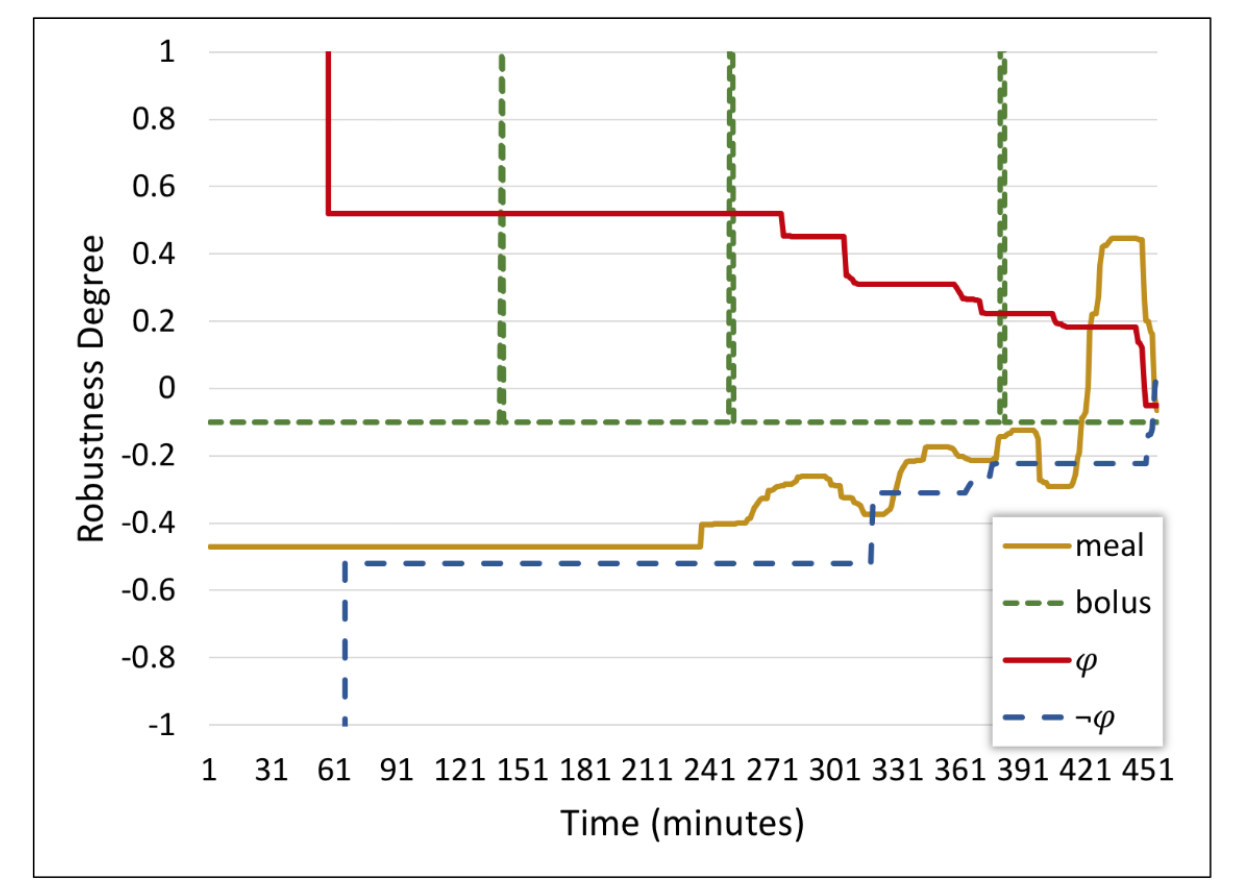
\includegraphics[width=0.4\textwidth]{t1d-patient}
    \end{figure}
    \begin{itemize}
        \item $t_1 = t_2 = 30 (minutes)$
        \item Plot shows $b_1$ for $\varphi$ and $a_2$ for $\neg\varphi$
        \item Meal occurs at $t=421$, but no bolus detected in
            $391 \leq t \leq 421$. Thus, when t slightly above $451$
            formula is \textit{rejected}, as $a_2 > \delta$.
        \item Noisy \textit{B (bolus)} signal, unobservable \textit{M (meal)}
            variable
    \end{itemize}
\end{frame}

\begin{frame}
    \frametitle{Example}
    \framesubtitle{Monitoring a Diabetic Patient}
    \begin{figure}[h]
        \centering
        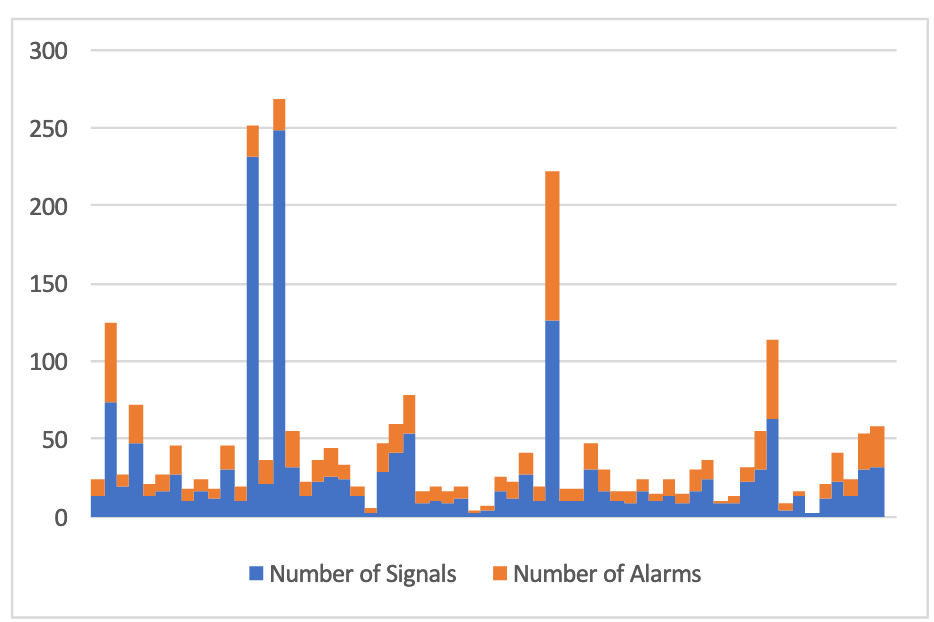
\includegraphics[width=0.4\textwidth]{false-alarms}
    \end{figure}
    \begin{itemize}
        \item Data for 61 patients, each monitored for different time lengths.
        \item Plot shows \textit{alarms} vs \textit{number of observations}
            for each patient.
        \item Evidence technique scales well for real world applications
    \end{itemize}
\end{frame}

\section{Conclusion}
\begin{frame}
    \frametitle{Conclusions}
    \begin{itemize}
        \item Introduce Parameteric Invariant Monitoring
            for Signal Temporal Logic
        \item Using \textit{robustness estimates} for
            single atomic propositions, derive \textit{robustness estimates}
            for entire formula.
        \item If \textit{robustness estimates} for
            atomic propositions is \textit{maximally invariant}
            then test procedure for entire formula is also
            \textit{maximally invariant} to nuissance paramters.
        \item Demonstrate real-world applications on monitoring
            an STL formula with patients having $T1-Diabetes$.
    \end{itemize}
\end{frame}














\end{document}

